% !TeX program = xelatex
\documentclass{article}
\usepackage{kotex}
\usepackage[a4paper,left=3cm, right=3cm, top=2cm, bottom=2cm]{geometry}
\usepackage{amsmath}
\usepackage{graphicx}
\usepackage{caption}
\usepackage{setspace}
\usepackage{xcolor}
\usepackage{titlesec}
\usepackage{amssymb}
\usepackage{tcolorbox}
\usepackage{amsthm}
\usepackage{multirow}
\usepackage{array}
\usepackage{booktabs}
\usepackage{tikz}
\usetikzlibrary{positioning,arrows.meta,calc,shapes.geometric}
\usepackage{pgfplots}
\pgfplotsset{compat=1.18}

\title{8.1 General Linear Transformations}
\date{}
\author{}
\setstretch{1.3}

\titleformat{name=\section, numberless}
  {\normalfont\large\bfseries\color{blue}}{}
  {0pt}{}
\geometry{a4paper, margin=1in}

\newcommand{\redheading}[1]{{\vspace{2mm}\noindent\Large\bfseries\color{red!55!black} #1\par}\vspace{2mm}}

\begin{document}
\maketitle

{\itshape\color{blue!45!black}
Up to now our study of linear transformations has focused on transformations from $R^n$
to $R^m$. In this section we turn our attention to linear transformations involving general
vector spaces, illustrate ways in which they arise, and establish a fundamental relationship
between general $n$-dimensional vector spaces and $R^n$.\par}

\vspace{2mm}

\redheading{Definitions and Terminology}

In Section~1.8 we defined a matrix transformation $T_A : R^n \to R^m$ as $T_A(\mathbf{x}) = A\mathbf{x}$.
We subsequently showed (Theorem~1.8.3) that matrix transformations are precisely the linear
transformations from $R^n$ to $R^m$, i.e., those satisfying
\[
  T(\mathbf{u}+\mathbf{v}) = T(\mathbf{u})+T(\mathbf{v}) \qquad \text{and} \qquad T(k\mathbf{u}) = kT(\mathbf{u})
\]
We use these two properties as the starting point for the following general definition.

\begin{tcolorbox}[colback=teal!4, colframe=teal!65!black,
  title={\textbf{Definition 1}}, boxrule=0.5mm, arc=3mm]
If $T : V \to W$ is a mapping from a vector space $V$ to a vector space $W$, then $T$ is
a \textbf{linear transformation} from $V$ to $W$ if for all vectors $\mathbf{u},\mathbf{v}$ in
$V$ and all scalars $k$:
\begin{enumerate}
  \item[(i)] $T(k\mathbf{u}) = kT(\mathbf{u})$ \hfill \textbf{[Homogeneity property]}
  \item[(ii)] $T(\mathbf{u}+\mathbf{v}) = T(\mathbf{u})+T(\mathbf{v})$ \hfill \textbf{[Additivity property]}
\end{enumerate}
When $V = W$, the linear transformation $T$ is called a \textbf{linear operator} on $V$.
\end{tcolorbox}

Combining the two properties shows that for any vectors $\mathbf{v}_1,\ldots,\mathbf{v}_n$ in $V$
and scalars $k_1,\ldots,k_n$,
\begin{equation}
  T(k_1\mathbf{v}_1 + k_2\mathbf{v}_2 + \cdots + k_n\mathbf{v}_n)
  = k_1 T(\mathbf{v}_1) + k_2 T(\mathbf{v}_2) + \cdots + k_n T(\mathbf{v}_n) \tag{1}
\end{equation}

\begin{tcolorbox}[colback=red!4, colframe=red!60!black,
  title={\textbf{Theorem 8.1.1}}, boxrule=0.5mm, arc=3mm]
If $T : V \to W$ is a linear transformation, then:
\begin{enumerate}
  \item[(a)] $T(\mathbf{0}) = \mathbf{0}$.
  \item[(b)] $T(\mathbf{u}-\mathbf{v}) = T(\mathbf{u}) - T(\mathbf{v})$ for all $\mathbf{u},\mathbf{v}$ in $V$.
  \item[(c)] $T(-\mathbf{v}) = -T(\mathbf{v})$ for all $\mathbf{v}$ in $V$.
\end{enumerate}
\end{tcolorbox}

\medskip
\textbf{Proof.} For (a): $T(\mathbf{0}) = T(0\mathbf{u}) = 0T(\mathbf{u}) = \mathbf{0}$.
For (b): $T(\mathbf{u}-\mathbf{v}) = T(\mathbf{u}+(-1)\mathbf{v}) = T(\mathbf{u})+(-1)T(\mathbf{v}) = T(\mathbf{u})-T(\mathbf{v})$.
Part (c) follows by setting $\mathbf{u}=\mathbf{0}$ in (b). $\blacksquare$

\subsection*{EXAMPLE 1 | Matrix Transformations}

Every matrix transformation $T_A : R^n \to R^m$ defined by $T_A(\mathbf{x}) = A\mathbf{x}$ is
a linear transformation (since matrix multiplication satisfies both homogeneity and
additivity).

\subsection*{EXAMPLE 2 | The Zero Transformation}

The mapping $T : V \to W$ defined by $T(\mathbf{v}) = \mathbf{0}$ for every $\mathbf{v}$ in $V$
is linear (the \textbf{zero transformation}), since
\[
  T(\mathbf{u}+\mathbf{v}) = \mathbf{0} = \mathbf{0}+\mathbf{0} = T(\mathbf{u})+T(\mathbf{v})
  \quad\text{and}\quad T(k\mathbf{u}) = \mathbf{0} = k\mathbf{0} = kT(\mathbf{u})
\]

\subsection*{EXAMPLE 3 | The Identity Operator}

The mapping $I : V \to V$ defined by $I(\mathbf{v}) = \mathbf{v}$ is a linear operator on $V$
(the \textbf{identity operator}).

\subsection*{EXAMPLE 4 | Dilation and Contraction Operators}

If $c$ is any scalar, the operator $T : V \to V$ defined by $T(\mathbf{x}) = c\mathbf{x}$ is
linear, since $T(k\mathbf{u}) = c(k\mathbf{u}) = k(c\mathbf{u}) = kT(\mathbf{u})$ and
$T(\mathbf{u}+\mathbf{v}) = c(\mathbf{u}+\mathbf{v}) = c\mathbf{u}+c\mathbf{v} = T(\mathbf{u})+T(\mathbf{v})$.
When $0 < c < 1$ this is called a \textbf{contraction} of $V$ with factor $c$; when $c > 1$,
a \textbf{dilation} of $V$ with factor $c$.

\subsection*{EXAMPLE 5 | A Linear Transformation from $P_n$ to $P_{n+1}$}

Let $\mathbf{p} = p(x) = c_0 + c_1 x + \cdots + c_n x^n \in P_n$ and define
$T : P_n \to P_{n+1}$ by $T(\mathbf{p}) = xp(x) = c_0 x + c_1 x^2 + \cdots + c_n x^{n+1}$.
For scalar $k$ and polynomials $\mathbf{p}_1, \mathbf{p}_2 \in P_n$:
\[
  T(k\mathbf{p}) = x(kp(x)) = k(xp(x)) = kT(\mathbf{p})
\]
\[
  T(\mathbf{p}_1+\mathbf{p}_2) = x(p_1(x)+p_2(x)) = xp_1(x)+xp_2(x) = T(\mathbf{p}_1)+T(\mathbf{p}_2)
\]
so $T$ is linear.

\subsection*{EXAMPLE 6 | A Linear Transformation Using an Inner Product}

Let $\mathbf{v}_0$ be any fixed vector in a real inner product space $V$, and define
$T : V \to R$ by $T(\mathbf{x}) = \langle \mathbf{x},\mathbf{v}_0\rangle$.
From properties of inner products:
\[
  T(k\mathbf{u}) = \langle k\mathbf{u},\mathbf{v}_0\rangle = k\langle\mathbf{u},\mathbf{v}_0\rangle = kT(\mathbf{u})
\]
\[
  T(\mathbf{u}+\mathbf{v}) = \langle\mathbf{u}+\mathbf{v},\mathbf{v}_0\rangle
  = \langle\mathbf{u},\mathbf{v}_0\rangle + \langle\mathbf{v},\mathbf{v}_0\rangle = T(\mathbf{u})+T(\mathbf{v})
\]

\subsection*{EXAMPLE 7 | Transformations on Matrix Spaces}

Let $M_{nn}$ be the space of $n\times n$ matrices. Determine whether the following are linear.

\noindent(a) $T_1(A) = A^T$ \quad (b) $T_2(A) = \det(A)$

\textbf{SOLUTION (a):} From properties of the transpose, $T_1(kA) = (kA)^T = kA^T = kT_1(A)$
and $T_1(A+B) = (A+B)^T = A^T+B^T = T_1(A)+T_1(B)$, so $T_1$ is linear.

\textbf{SOLUTION (b):} $T_2(kA) = \det(kA) = k^n\det(A) = k^n T_2(A)$, which is not $kT_2(A)$
for $n>1$. Also, $\det(A+B) \neq \det A + \det B$ in general (Section~2.3). So $T_2$ is not linear.

\subsection*{EXAMPLE 8 | Translation Is Not Linear}

If $\mathbf{x}_0$ is a fixed nonzero vector in $V$, the transformation $T(\mathbf{x}) = \mathbf{x}+\mathbf{x}_0$
is \emph{not} linear, since $T(\mathbf{0}) = \mathbf{x}_0 \neq \mathbf{0}$
(violating part (a) of Theorem~8.1.1). Geometrically, this \textbf{translation} shifts
each point $\mathbf{x}$ along a line parallel to $\mathbf{x}_0$ through distance $\|\mathbf{x}_0\|$.

\begin{figure}[ht]
\centering
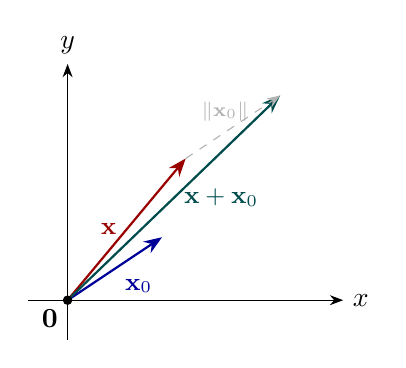
\begin{tikzpicture}[>=Stealth, scale=1.0]
  \draw[->] (-0.5,0)--(3.5,0) node[right]{$x$};
  \draw[->] (0,-0.5)--(0,3.0) node[above]{$y$};
  % x0 vector
  \draw[->, thick, blue!60!black] (0,0) -- (1.2,0.8)
    node[midway, below right, font=\small]{$\mathbf{x}_0$};
  % x vector
  \draw[->, thick, red!60!black] (0,0) -- (1.5,1.8)
    node[midway, left, font=\small]{$\mathbf{x}$};
  % x + x0 vector
  \draw[->, thick, teal!60!black] (0,0) -- (2.7,2.6)
    node[midway, right, font=\small]{$\mathbf{x}+\mathbf{x}_0$};
  % dashed translation arrow
  \draw[->, dashed, gray!60] (1.5,1.8) -- (2.7,2.6);
  \node[font=\scriptsize, gray!60] at (2.0,2.4) {$\|\mathbf{x}_0\|$};
  \filldraw[black] (0,0) circle (1.5pt) node[below left]{$\mathbf{0}$};
\end{tikzpicture}
\caption*{FIGURE 8.1.1\quad $T(\mathbf{x}) = \mathbf{x}+\mathbf{x}_0$ translates each point along
a line parallel to $\mathbf{x}_0$ through distance $\|\mathbf{x}_0\|$.}
\end{figure}

\subsection*{EXAMPLE 9 | The Evaluation Transformation}

Let $V$ be a subspace of $F(-\infty,\infty)$, let $x_1,x_2,\ldots,x_n$ be distinct real
numbers, and define $T : V \to R^n$ by
\[
  T(f) = (f(x_1), f(x_2), \ldots, f(x_n)) \tag{2}
\]
This \textbf{evaluation transformation} is linear. For example, if $x_1=-1$, $x_2=2$, $x_3=4$
and $f(x)=x^2-1$, then $T(f) = (f(-1), f(2), f(4)) = (0,3,15)$. Linearity follows from
$T(kf) = k(f(x_1),\ldots,f(x_n)) = kT(f)$ and $T(f+g) = T(f)+T(g)$.

\vspace{2mm}

\redheading{Finding Linear Transformations from Images of Basis Vectors}

For a matrix transformation $T_A : R^n \to R^m$ with standard basis $\mathbf{e}_1,\ldots,\mathbf{e}_n$,
any image $T_A(\mathbf{v}) = c_1 T_A(\mathbf{e}_1)+\cdots+c_n T_A(\mathbf{e}_n)$ is determined
by the images of the basis vectors. The following theorem extends this to general vector spaces.

\begin{tcolorbox}[colback=red!4, colframe=red!60!black,
  title={\textbf{Theorem 8.1.2}}, boxrule=0.5mm, arc=3mm]
Let $T : V \to W$ be a linear transformation with $V$ finite-dimensional. If
$S = \{\mathbf{v}_1,\mathbf{v}_2,\ldots,\mathbf{v}_n\}$ is a basis for $V$, then for any $\mathbf{v}$
in $V$:
\[
  T(\mathbf{v}) = c_1 T(\mathbf{v}_1) + c_2 T(\mathbf{v}_2) + \cdots + c_n T(\mathbf{v}_n) \tag{3}
\]
where $c_1,c_2,\ldots,c_n$ are the coordinates of $\mathbf{v}$ relative to $S$.
\end{tcolorbox}

\medskip
\textbf{Proof.} Write $\mathbf{v} = c_1\mathbf{v}_1+\cdots+c_n\mathbf{v}_n$ and apply linearity
of $T$. $\blacksquare$

\subsection*{EXAMPLE 10 | Computing with Images of Basis Vectors}

Let $S = \{\mathbf{v}_1,\mathbf{v}_2,\mathbf{v}_3\}$ for $R^3$, where
$\mathbf{v}_1=(1,1,1)$, $\mathbf{v}_2=(1,1,0)$, $\mathbf{v}_3=(1,0,0)$.
Let $T : R^3 \to R^2$ be linear with
$T(\mathbf{v}_1)=(1,0)$, $T(\mathbf{v}_2)=(2,-1)$, $T(\mathbf{v}_3)=(4,3)$.
Find a formula for $T(x_1,x_2,x_3)$, then compute $T(2,-3,5)$.

\textbf{SOLUTION:} Write $(x_1,x_2,x_3) = c_1(1,1,1)+c_2(1,1,0)+c_3(1,0,0)$; solving gives
$c_1=x_3$, $c_2=x_2-x_3$, $c_3=x_1-x_2$. By Theorem~8.1.2:
\begin{align*}
  T(x_1,x_2,x_3) &= x_3(1,0)+(x_2-x_3)(2,-1)+(x_1-x_2)(4,3)\\
                  &= (4x_1-2x_2-x_3,\; 3x_1-4x_2+x_3)
\end{align*}
Thus $T(2,-3,5) = (4(2)-2(-3)-5,\; 3(2)-4(-3)+5) = (9,23)$.

\subsection*{EXAMPLE 11 | A Linear Transformation from $C^1(-\infty,\infty)$ to $F(-\infty,\infty)$}
\textit{(Calculus Required)}

Let $V=C^1(-\infty,\infty)$ and $W=F(-\infty,\infty)$, and define $D : V \to W$ by
$D(\mathbf{f}) = f'(x)$ (the differentiation operator). From calculus:
\[
  D(\mathbf{f}+\mathbf{g}) = D(\mathbf{f})+D(\mathbf{g}) \qquad \text{and} \qquad D(k\mathbf{f}) = kD(\mathbf{f})
\]
so $D$ is a linear transformation.

\subsection*{EXAMPLE 12 | An Integral Transformation}
\textit{(Calculus Required)}

Let $V=C(-\infty,\infty)$, $W=C^1(-\infty,\infty)$, and define $J : V \to W$ by
$J(f) = \displaystyle\int_0^x f(t)\,dt$. For example, if $f(x)=x^2$:
\[
  J(f) = \int_0^x t^2\,dt = \frac{t^3}{3}\Bigr|_0^x = \frac{x^3}{3}
\]
Linearity follows from properties of the integral: $J(kf) = k\!\int_0^x\! f = kJ(f)$ and
$J(f+g) = \int_0^x(f+g) = J(f)+J(g)$.

\vspace{2mm}

\redheading{Kernel and Range}

For a matrix transformation $T_A$, the null space of $A$ consists of all vectors mapped to
$\mathbf{0}$, and the column space consists of all images. The following definition extends
these concepts.

\begin{tcolorbox}[colback=teal!4, colframe=teal!65!black,
  title={\textbf{Definition 2}}, boxrule=0.5mm, arc=3mm]
If $T : V \to W$ is a linear transformation, then the \textbf{kernel} of $T$ is
\[
  \ker(T) = \{\mathbf{v}\in V : T(\mathbf{v}) = \mathbf{0}\}
\]
and the \textbf{range} of $T$ is
\[
  R(T) = \{\mathbf{w}\in W : \mathbf{w} = T(\mathbf{v})\text{ for some }\mathbf{v}\in V\}
\]
\end{tcolorbox}

\begin{figure}[ht]
\centering
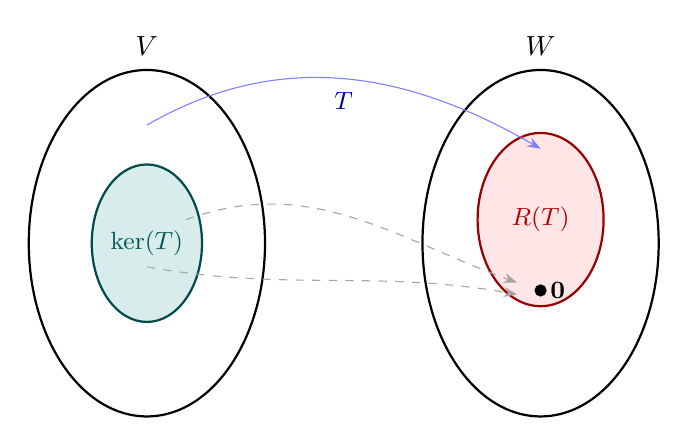
\begin{tikzpicture}[>=Stealth, scale=1.0]
  % V ellipse
  \draw[thick] (-2.5,0) ellipse (1.5 and 2.2);
  \node at (-2.5, 2.5) {$V$};
  % kernel region inside V
  \fill[teal!15] (-2.5,0) ellipse (0.7 and 1.0);
  \draw[thick, teal!60!black] (-2.5,0) ellipse (0.7 and 1.0);
  \node[font=\small, teal!70!black] at (-2.5,0) {$\ker(T)$};
  % W ellipse
  \draw[thick] (2.5,0) ellipse (1.5 and 2.2);
  \node at (2.5, 2.5) {$W$};
  % R(T) region inside W
  \fill[red!10] (2.5,0.3) ellipse (0.8 and 1.1);
  \draw[thick, red!60!black] (2.5,0.3) ellipse (0.8 and 1.1);
  \node[font=\small, red!70!black] at (2.5,0.3) {$R(T)$};
  % zero in W
  \filldraw[black] (2.5,-0.6) circle (2pt) node[right, font=\small]{$\mathbf{0}$};
  % arrows from ker(T) to 0
  \draw[->, gray!70, dashed] (-2.0,0.3) to[out=20, in=160] (2.2,-0.5);
  \draw[->, gray!70, dashed] (-2.5,-0.3) to[out=-10, in=170] (2.2,-0.65);
  % arrow from outside ker to R(T)
  \draw[->, blue!50] (-2.5,1.5) to[out=30, in=150] (2.5,1.2);
  \node[font=\small, blue!60!black] at (0, 1.8) {$T$};
\end{tikzpicture}
\caption*{FIGURE 8.1.2\quad The kernel maps to $\mathbf{0}$; the range is the set of all
images.}
\end{figure}

\subsection*{EXAMPLE 13 | Kernel and Range of a Matrix Transformation}

If $T_A : R^n \to R^m$ is multiplication by $m\times n$ matrix $A$, then $\ker(T_A)$ is
the null space of $A$ and $R(T_A)$ is the column space of $A$.

\subsection*{EXAMPLE 14 | Kernel and Range of the Zero Transformation}

For the zero transformation $T : V \to W$: $T$ maps every vector to $\mathbf{0}$, so
$\ker(T) = V$. Since $\mathbf{0}$ is the only image, $R(T) = \{\mathbf{0}\}$.

\subsection*{EXAMPLE 15 | Kernel and Range of the Identity Operator}

For $I : V \to V$: every vector is its own image so $R(I) = V$, and the only vector mapped
to $\mathbf{0}$ is $\mathbf{0}$ itself, so $\ker(I) = \{\mathbf{0}\}$.

\subsection*{EXAMPLE 16 | Kernel and Range of an Orthogonal Projection}

Let $T : R^3 \to R^3$ be the orthogonal projection onto the $xy$-plane: $T(x,y,z) = (x,y,0)$.
The points mapped to $\mathbf{0} = (0,0,0)$ are those of the form $(0,0,z)$, so
$\ker(T)$ is the $z$-axis. Every point in the $xy$-plane is the image of each point on the
vertical line above it, so $R(T)$ is the entire $xy$-plane.

\begin{figure}[ht]
\centering
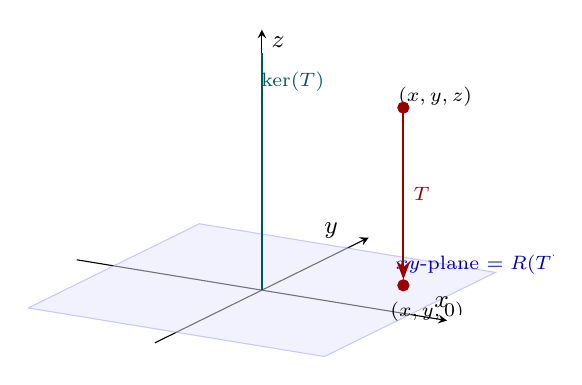
\begin{tikzpicture}[>=Stealth]
\begin{axis}[
  width=9cm, height=7cm,
  view={30}{25},
  axis lines=center,
  xlabel={$x$}, ylabel={$y$}, zlabel={$z$},
  ticks=none,
  xmin=-1.5, xmax=1.5,
  ymin=-1.5, ymax=1.5,
  zmin=0, zmax=2.2,
  xlabel style={font=\small},
  ylabel style={font=\small},
  zlabel style={font=\small},
]
  % xy-plane shaded
  \addplot3[fill=blue!10, opacity=0.5, draw=blue!40]
    coordinates{(-1.2,-1.2,0)(1.2,-1.2,0)(1.2,1.2,0)(-1.2,1.2,0)(-1.2,-1.2,0)};
  \node[font=\scriptsize, blue!70!black] at (axis cs:1.0,1.3,0) {$xy$-plane $= R(T)$};
  % z-axis highlighted as ker(T)
  \addplot3[thick, teal!70!black, domain=0:2, samples=2, variable=\t]
    ({0},{0},{\t});
  \node[font=\scriptsize, teal!70!black] at (axis cs:0.25,0,1.8) {$\ker(T)$};
  % a sample point and its projection
  \addplot3[mark=*, mark size=2pt, red!60!black]
    coordinates{(0.8,0.6,1.5)};
  \node[font=\scriptsize] at (axis cs:1.0,0.7,1.6) {$(x,y,z)$};
  \addplot3[mark=*, mark size=2pt, red!60!black]
    coordinates{(0.8,0.6,0)};
  \node[font=\scriptsize] at (axis cs:1.05,0.5,-0.15) {$(x,y,0)$};
  \draw[->, thick, red!60!black]
    (axis cs:0.8,0.6,1.5) -- (axis cs:0.8,0.6,0.05)
    node[midway, right, font=\scriptsize]{$T$};
\end{axis}
\end{tikzpicture}
\caption*{FIGURE 8.1.3\quad Projection onto the $xy$-plane: $\ker(T)$ is the $z$-axis and
$R(T)$ is the $xy$-plane.}
\end{figure}

\subsection*{EXAMPLE 17 | Kernel and Range of a Rotation}

Let $T : R^2 \to R^2$ rotate each vector through angle $\theta$. Since every vector in the
$xy$-plane can be obtained by rotating some vector through $\theta$, we have $R(T) = R^2$.
The only vector that rotates into $\mathbf{0}$ is $\mathbf{0}$ itself, so $\ker(T) = \{\mathbf{0}\}$.

\begin{figure}[ht]
\centering
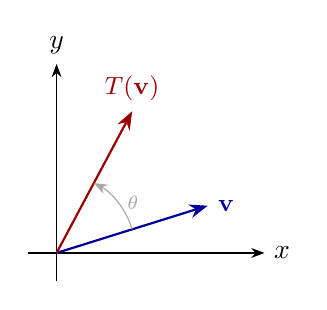
\begin{tikzpicture}[>=Stealth, scale=1.2]
  \draw[->] (-0.3,0)--(2.2,0) node[right]{$x$};
  \draw[->] (0,-0.3)--(0,2.0) node[above]{$y$};
  % v vector
  \draw[->, thick, blue!60!black] (0,0) -- (1.6,0.5)
    node[right, font=\small]{$\mathbf{v}$};
  % T(v) vector (rotated by theta)
  \draw[->, thick, red!60!black] (0,0) -- (0.8,1.5)
    node[above, font=\small]{$T(\mathbf{v})$};
  % arc showing theta
  \draw[->, gray!70] (0.8,0.25) arc[start angle=17, end angle=62, radius=0.83]
    node[midway, right, font=\scriptsize]{$\theta$};
\end{tikzpicture}
\caption*{FIGURE 8.1.4\quad Rotation by $\theta$: $\ker(T)=\{\mathbf{0}\}$, $R(T)=R^2$.}
\end{figure}

\subsection*{EXAMPLE 18 | Kernel of a Differentiation Transformation}
\textit{(Calculus Required)}

For the differentiation operator $D : C^1(-\infty,\infty) \to F(-\infty,\infty)$ defined
by $D(\mathbf{f}) = f'(x)$, the kernel consists of all functions with zero derivative,
which is the set of constant functions on $(-\infty,\infty)$.

\subsection*{EXAMPLE 19 | Application to Differential Equations}
\textit{(Calculus Required)}

Differential equations of the form
\[
  y'' + \omega^2 y = 0 \qquad (\omega \text{ a positive constant}) \tag{5}
\]
arise in the study of vibrations. The set of all solutions on $(-\infty,\infty)$ is the
kernel of $D : C^2(-\infty,\infty) \to C(-\infty,\infty)$ defined by $D(y) = y''+\omega^2 y$.
It can be shown that $y_1 = \cos\omega x$ and $y_2 = \sin\omega x$ are two linearly
independent solutions of~(5), so the kernel is a 2-dimensional subspace and every solution
has the form
\[
  y = c_1 \cos\omega x + c_2 \sin\omega x \tag{6}
\]

\vspace{2mm}

\redheading{Properties of Kernel and Range}

In all of the preceding examples $\ker(T)$ and $R(T)$ turned out to be subspaces.
This is always the case.

\begin{tcolorbox}[colback=red!4, colframe=red!60!black,
  title={\textbf{Theorem 8.1.3}}, boxrule=0.5mm, arc=3mm]
If $T : V \to W$ is a linear transformation, then:
\begin{enumerate}
  \item[(a)] The kernel of $T$ is a subspace of $V$.
  \item[(b)] The range of $T$ is a subspace of $W$.
\end{enumerate}
\end{tcolorbox}

\medskip
\textbf{Proof of (a).} By Theorem~8.1.1(a), $\mathbf{0} \in \ker(T)$. If $\mathbf{v}_1,\mathbf{v}_2
\in \ker(T)$ and $k$ is any scalar, then
\[
  T(\mathbf{v}_1+\mathbf{v}_2) = T(\mathbf{v}_1)+T(\mathbf{v}_2) = \mathbf{0}+\mathbf{0} = \mathbf{0}
\]
\[
  T(k\mathbf{v}_1) = kT(\mathbf{v}_1) = k\mathbf{0} = \mathbf{0}
\]
so $\ker(T)$ is closed under addition and scalar multiplication. $\blacksquare$

\medskip
\textbf{Proof of (b).} Since $T(\mathbf{0})=\mathbf{0}$, we have $\mathbf{0}\in R(T)$.
If $\mathbf{w}_1,\mathbf{w}_2\in R(T)$ and $k$ is any scalar, there exist $\mathbf{v}_1,\mathbf{v}_2$
in $V$ with $T(\mathbf{v}_i)=\mathbf{w}_i$. Then
\[
  T(\mathbf{v}_1+\mathbf{v}_2) = \mathbf{w}_1+\mathbf{w}_2, \quad T(k\mathbf{v}_1) = k\mathbf{w}_1
\]
so $\mathbf{w}_1+\mathbf{w}_2 \in R(T)$ and $k\mathbf{w}_1 \in R(T)$. $\blacksquare$

\vspace{2mm}

\redheading{Rank and Nullity of Linear Transformations}

In Section~4.9 we defined rank and nullity for $m\times n$ matrices. These concepts extend
to general linear transformations.

\begin{tcolorbox}[colback=teal!4, colframe=teal!65!black,
  title={\textbf{Definition 3}}, boxrule=0.5mm, arc=3mm]
Let $T : V \to W$ be a linear transformation. If $R(T)$ is finite-dimensional, its
dimension is called the \textbf{rank} of $T$. If $\ker(T)$ is finite-dimensional, its
dimension is called the \textbf{nullity} of $T$. These are denoted
\[
  \text{rank}(T) \qquad \text{and} \qquad \text{nullity}(T)
\]
\end{tcolorbox}

\begin{tcolorbox}[colback=red!4, colframe=red!60!black,
  title={\textbf{Theorem 8.1.4 --- Dimension Theorem for Linear Transformations}},
  boxrule=0.5mm, arc=3mm]
If $T : V \to W$ is a linear transformation from a finite-dimensional vector space $V$
to a vector space $W$, then the range of $T$ is finite-dimensional and
\begin{equation}
  \text{rank}(T) + \text{nullity}(T) = \dim(V) \tag{7}
\end{equation}
\end{tcolorbox}

For the special case $T_A : R^n \to R^m$ (multiplication by $A$), $\ker(T_A)$ is the null
space of $A$ and $R(T_A)$ is the column space of $A$, so Theorem~8.1.4 gives the familiar
result $\text{rank}(T_A) + \text{nullity}(T_A) = n$.

\vspace{3mm}
\noindent\rule{\linewidth}{0.5pt}

\section*{Exercise Set 8.1}

\noindent\textit{In Exercises 1--2, suppose $T$ is a mapping whose domain is the vector
space $M_{22}$. Determine whether $T$ is a linear transformation, and if so, find its kernel.}

\begin{enumerate}

  \item \textbf{a.} $T(A) = A^2$ \quad \textbf{b.} $T(A) = \mathrm{tr}(A)$ \quad
        \textbf{c.} $T(A) = A + A^T$

  \item[3.] $T : R^3 \to R$, where $T(\mathbf{u}) = \|\mathbf{u}\|$.

  \item[4.] $T : R^3 \to R^3$, where $\mathbf{v}_0$ is a fixed vector in $R^3$ and
        $T(\mathbf{u}) = \mathbf{u}\times\mathbf{v}_0$.

  \item[5.] $T : M_{22} \to M_{23}$, where $B$ is a fixed $2\times 3$ matrix and $T(A) = AB$.

  \item[7.] $T : P_2 \to P_2$, where \\
        \textbf{a.} $T(a_0+a_1x+a_2x^2) = a_0 + a_1(x+1) + a_2(x+1)^2$\\
        \textbf{b.} $T(a_0+a_1x+a_2x^2) = (a_0+1)+(a_1+1)x+(a_2+1)x^2$

\end{enumerate}

\noindent\textit{In Exercises 10--11, $T : P_2 \to P_3$ is defined by $T(p(x)) = xp(x)$.}

\begin{enumerate}
  \item[10.] Which of the following are in $\ker(T)$?
        \quad \textbf{a.}~$x^2$ \quad \textbf{b.}~$0$ \quad \textbf{c.}~$1+x$ \quad \textbf{d.}~$-x$

  \item[11.] Which of the following are in $R(T)$?
        \quad \textbf{a.}~$x+x^2$ \quad \textbf{b.}~$1+x$ \quad \textbf{c.}~$3-x^2$ \quad \textbf{d.}~$-x$

  \item[12.] Let $V$ be any vector space and $T : V \to V$ defined by $T(\mathbf{v}) = 3\mathbf{v}$.\\
        \textbf{a.} What is $\ker(T)$? \quad \textbf{b.} What is $R(T)$?

  \item[13.] Use the given information to find the nullity of $T$.\\
        \textbf{a.} $T : R^5 \to P_5$ has rank 3. \quad
        \textbf{b.} $T : P_4 \to P_3$ has rank 1. \quad
        \textbf{c.} The range of $T : M_{mn} \to R^3$ is $R^3$.\\
        \textbf{d.} $T : M_{22} \to M_{22}$ has rank 3.

  \item[15.] Let $T : M_{22} \to M_{22}$ be the dilation operator with factor $k = 3$.\\
        \textbf{a.} Find $T\!\left(\begin{bmatrix}1&2\\-4&3\end{bmatrix}\right)$.
        \quad \textbf{b.} Find the rank and nullity of $T$.

  \item[17.] Let $T : P_2 \to R^3$ be the evaluation transformation at
        $x_1=-1$, $x_2=0$, $x_3=1$.\\
        \textbf{a.} Find $T(x^2)$. \quad
        \textbf{b.} Find $\ker(T)$. \quad
        \textbf{c.} Find $R(T)$.

\end{enumerate}

\noindent\textit{In Exercises 19--22, consider the basis $S = \{\mathbf{v}_1, \mathbf{v}_2\}$
(or $S=\{\mathbf{v}_1,\mathbf{v}_2,\mathbf{v}_3\}$) as given, and find a formula for
$T(x_1,x_2)$ (or $T(x_1,x_2,x_3)$) using the stated images.}

\begin{enumerate}
  \item[19.] $S = \{\mathbf{v}_1,\mathbf{v}_2\}$ for $R^2$: $\mathbf{v}_1=(1,1)$,
        $\mathbf{v}_2=(1,0)$; $T : R^2 \to R^2$ linear with
        $T(\mathbf{v}_1)=(1,-2)$, $T(\mathbf{v}_2)=(-4,1)$. Find $T(5,-3)$.

  \item[21.] $S=\{\mathbf{v}_1,\mathbf{v}_2,\mathbf{v}_3\}$ for $R^3$:
        $\mathbf{v}_1=(1,1,1)$, $\mathbf{v}_2=(1,1,0)$, $\mathbf{v}_3=(1,0,0)$;
        $T : R^3 \to R^3$ linear with $T(\mathbf{v}_1)=(2,-1,4)$,
        $T(\mathbf{v}_2)=(3,0,1)$, $T(\mathbf{v}_3)=(-1,5,1)$.
        Find $T(x_1,x_2,x_3)$ and $T(2,4,-1)$.

\end{enumerate}

\noindent\textit{In Exercises 23--24, let $T_A : R^n \to R^3$ be multiplication by $A$.
Find (a) a basis for the range of $T$, (b) a basis for the kernel of $T$,
(c) the rank and nullity of $T$, (d) the rank and nullity of $A$.}

\begin{enumerate}
  \item[23.] $A = \begin{bmatrix}1&-1&3\\5&6&-4\\7&4&2\end{bmatrix}$

  \item[24.] $A = \begin{bmatrix}2&0&-1\\4&0&-2\\20&0&0\end{bmatrix}$

\end{enumerate}

\noindent\textit{In Exercises 27--28, determine whether $T$ is linear, find a basis for
the kernel, and find a basis for the range.}

\begin{enumerate}
  \item[27.] $T : P_3 \to P_2$ defined by
        $T(a_0+a_1x+a_2x^2+a_3x^3) = 5a_0 + a_3x^2$.\\
        \textbf{a.} Show $T$ is linear. \quad
        \textbf{b.} Find a basis for $\ker(T)$. \quad
        \textbf{c.} Find a basis for $R(T)$.

  \item[28.] $T : P_2 \to P_2$ defined by
        $T(a_0+a_1x+a_2x^2) = 3a_0+a_1x+(a_0+a_1)x^2$.\\
        \textbf{a.} Show $T$ is linear. \quad
        \textbf{b.} Find a basis for $\ker(T)$. \quad
        \textbf{c.} Find a basis for $R(T)$.

  \item[32.] Let $T : M_{nn} \to R$ be defined by $T(A) = \mathrm{tr}(A)$, where $A$ is
        an $n\times n$ matrix with real entries.
        Determine the dimension of the range of $T$.

  \item[35.] Let $\mathbf{v}_1$, $\mathbf{v}_2$, $\mathbf{v}_3$ be vectors in a vector space
        $V$, and let $T : V \to R^3$ be a linear transformation for which
        \[
          T(\mathbf{v}_1)=(1,-1,2),\quad T(\mathbf{v}_2)=(0,3,2),\quad T(\mathbf{v}_3)=(-3,1,2)
        \]
        Find $T(2\mathbf{v}_1-3\mathbf{v}_2+4\mathbf{v}_3)$.

\end{enumerate}

\noindent\textit{Working with Proofs}

\begin{enumerate}
  \item[36.] Let $\{\mathbf{v}_1,\mathbf{v}_2,\ldots,\mathbf{v}_n\}$ be a basis for $V$ and
        $T : V \to W$ a linear transformation. Prove: if $T(\mathbf{v}_1)=T(\mathbf{v}_2)
        =\cdots=T(\mathbf{v}_n)=\mathbf{0}$, then $T$ is the zero transformation.

  \item[38.] Prove: if $\{\mathbf{v}_1,\mathbf{v}_2,\ldots,\mathbf{v}_n\}$ is a basis for $V$
        and $\mathbf{w}_1,\mathbf{w}_2,\ldots,\mathbf{w}_n$ are any vectors in $W$
        (not necessarily distinct), then there exists a unique linear transformation
        $T : V \to W$ such that $T(\mathbf{v}_k)=\mathbf{w}_k$ for $k=1,2,\ldots,n$.

\end{enumerate}

\end{document}
